\chapter{Implémentation}

\section{Résultats}

\subsection{Analyse exploratoire des données}

Le jeu de données nettoyé compte 603 annonces et 11 colonnes (identifiant, titre, catégorie,
prix, devise, quartier, ville/région, nombre de chambres, surface, date de publication, URL).
La répartition géographique est fortement concentrée : 515 annonces à Dakar (85{,}4~\%), 84 à
Thiès (13{,}9~\%), et seulement 4 annonces réparties entre Kaolack, Saint-Louis et d'autres
localités. Cette concentration reflète la structure même du marché des annonces en ligne au
Sénégal, très majoritairement actif dans la capitale, et constitue une limite explicite à la
capacité de généralisation du modèle en dehors de Dakar et Thiès, discutée en
\S~4.1.4.

\begin{figure}[ht]
  \centering
  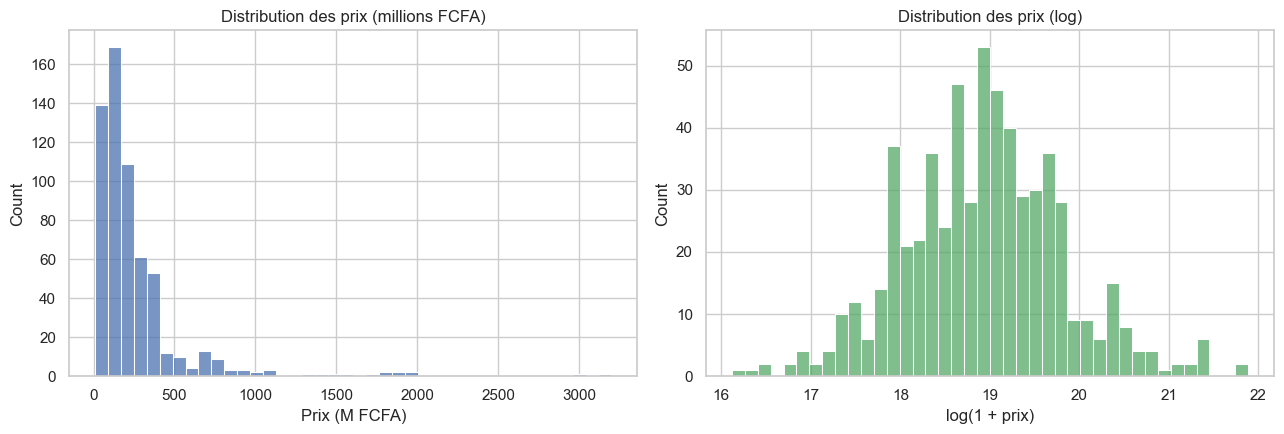
\includegraphics[width=0.95\textwidth]{figures/eda_01.png}
  \caption{Distribution des prix (échelle brute et échelle logarithmique)}
  \label{fig:eda-distribution}
\end{figure}

La distribution des prix (Figure~\ref{fig:eda-distribution}) est fortement asymétrique à droite,
avec une majorité de biens sous 300 millions FCFA et une longue traîne de biens haut de gamme.
Cette asymétrie justifie la transformation logarithmique de la cible retenue en \S~3.6.

\begin{figure}[ht]
  \centering
  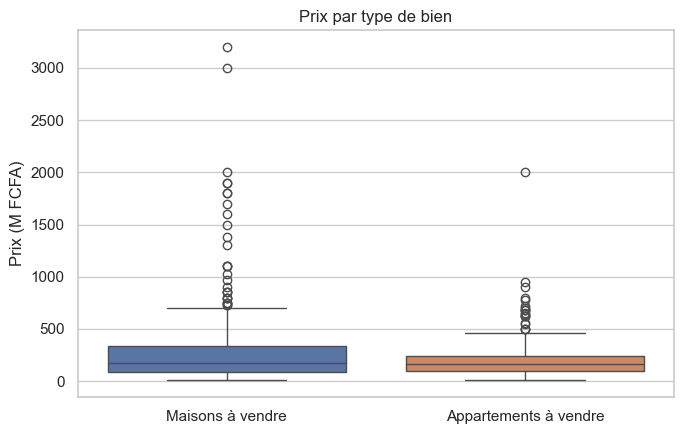
\includegraphics[width=0.75\textwidth]{figures/eda_02.png}
  \caption{Prix par type de bien (maison / appartement)}
  \label{fig:eda-category}
\end{figure}

\begin{figure}[ht]
  \centering
  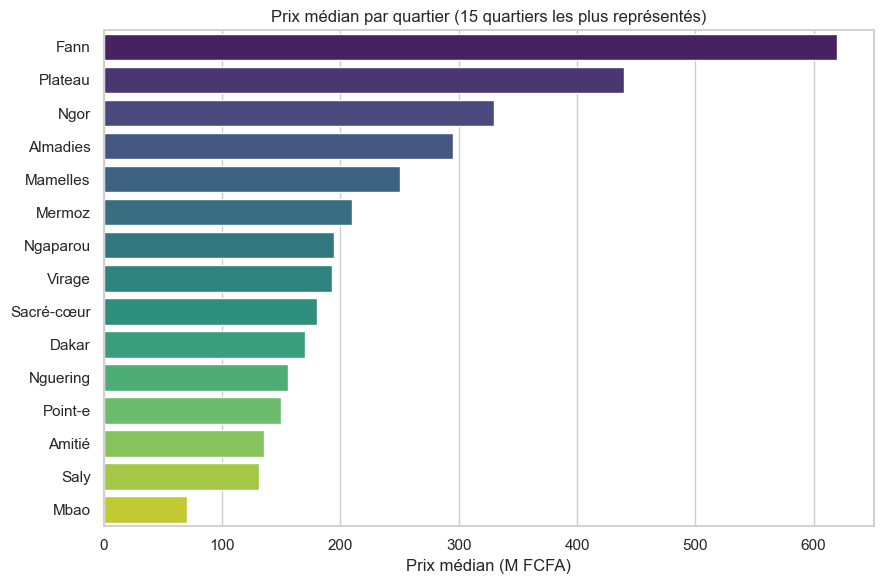
\includegraphics[width=0.85\textwidth]{figures/eda_03.png}
  \caption{Prix médian par quartier (15 quartiers les plus représentés)}
  \label{fig:eda-neighborhood}
\end{figure}

Le prix médian varie fortement selon le quartier (Figure~\ref{fig:eda-neighborhood}), les
quartiers résidentiels haut de gamme de Dakar (Almadies, Ngor, Mermoz) affichant des médianes
nettement supérieures à celles des quartiers périphériques, un résultat cohérent avec la
littérature sur le rôle central de la localisation dans la formation des prix
\citep{nwankwo2023lagos}.

\begin{figure}[ht]
  \centering
  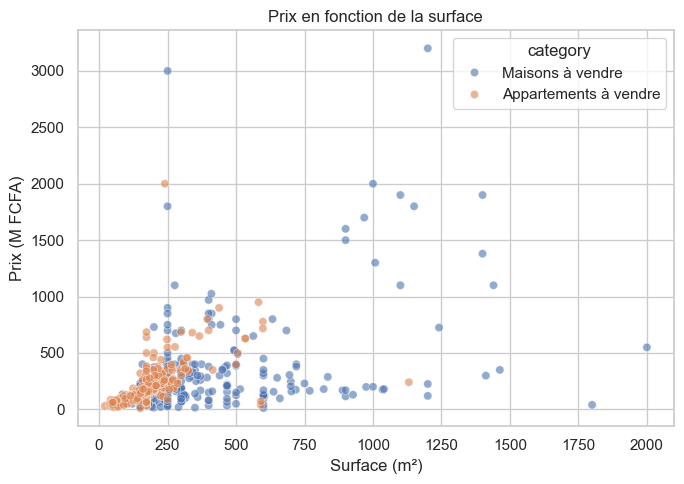
\includegraphics[width=0.75\textwidth]{figures/eda_04.png}
  \caption{Prix en fonction de la surface, par type de bien}
  \label{fig:eda-surface}
\end{figure}

\begin{figure}[ht]
  \centering
  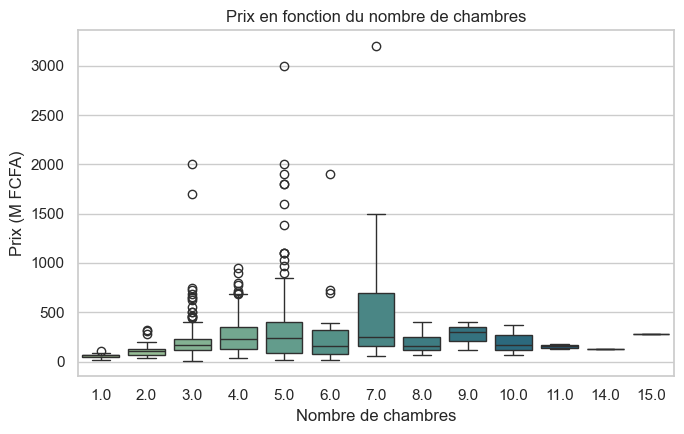
\includegraphics[width=0.75\textwidth]{figures/eda_05.png}
  \caption{Prix en fonction du nombre de chambres}
  \label{fig:eda-bedrooms}
\end{figure}

\begin{figure}[ht]
  \centering
  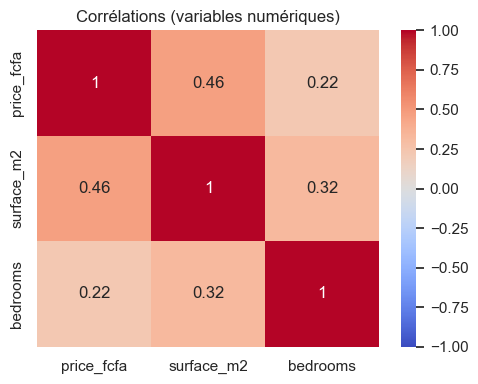
\includegraphics[width=0.55\textwidth]{figures/eda_06.png}
  \caption{Corrélations entre variables numériques}
  \label{fig:eda-corr}
\end{figure}

La surface (Figure~\ref{fig:eda-surface}) présente la relation la plus nette avec le prix, ce
que confirme la matrice de corrélation (Figure~\ref{fig:eda-corr}). Le nombre de chambres
(Figure~\ref{fig:eda-bedrooms}) a un effet positif mais plus diffus : des biens au nombre de
chambres identique peuvent présenter des surfaces, et donc des prix, très différents.

\subsection{Résultats des modèles}

Le tableau~\ref{tab:resultats} présente les performances des quatre modèles sur le jeu de test
(121 annonces), après optimisation des hyperparamètres pour Random Forest, XGBoost et le MLP.

\begin{table}[ht]
\centering
\caption{Performances comparées des modèles sur le jeu de test}
\label{tab:resultats}
\begin{tabular}{@{}lrrrr@{}}
\toprule
\textbf{Modèle} & \textbf{RMSE (FCFA)} & \textbf{MAE (FCFA)} & \textbf{MAPE (\%)} & \textbf{$R^2$} \\
\midrule
Régression linéaire        & 148\,156\,086 & 89\,002\,102 & 39{,}7 & 0{,}571 \\
Random Forest (optimisé)   & \textbf{112\,897\,339} & \textbf{73\,325\,765} & \textbf{34{,}0} & \textbf{0{,}751} \\
XGBoost (optimisé)         & 125\,455\,687 & 79\,242\,132 & 37{,}7 & 0{,}692 \\
MLP (optimisé)             & 125\,968\,083 & 82\,416\,154 & 37{,}0 & 0{,}690 \\
\bottomrule
\end{tabular}
\end{table}

Les meilleurs hyperparamètres retenus par la recherche aléatoire sont : pour Random Forest,
\texttt{n\_estimators=400}, \texttt{max\_depth=30}, \texttt{min\_samples\_split=5},
\texttt{min\_samples\_leaf=1}, \texttt{max\_features='log2'} ; pour XGBoost,
\texttt{n\_estimators=300}, \texttt{max\_depth=3}, \texttt{learning\_rate=0.1},
\texttt{subsample=1.0}, \texttt{colsample\_bytree=0.6}, \texttt{reg\_alpha=0.1},
\texttt{reg\_lambda=1} ; pour le MLP, \texttt{hidden\_layer\_sizes=(32,)},
\texttt{activation='tanh'}, \texttt{alpha=0.1}, \texttt{learning\_rate\_init=0.005}.

\begin{figure}[ht]
  \centering
  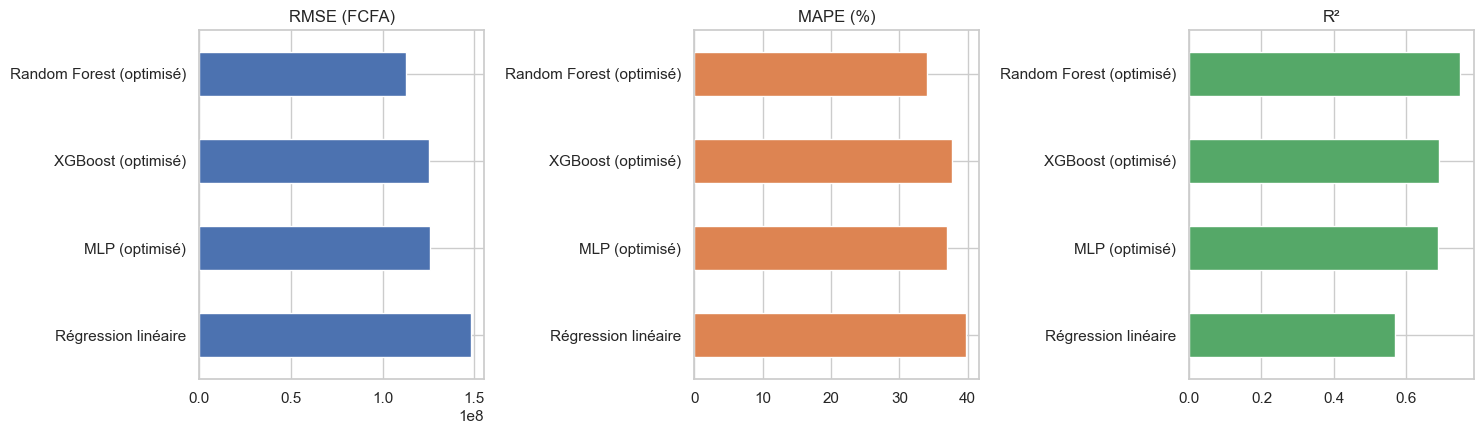
\includegraphics[width=0.95\textwidth]{figures/model_01.png}
  \caption{Comparaison visuelle des modèles (RMSE, MAPE, $R^2$)}
  \label{fig:model-comparison}
\end{figure}

\subsection{Interprétation des résultats}

Random Forest domine nettement les trois autres modèles sur les quatre métriques
(Figure~\ref{fig:model-comparison}), avec un gain de MAE de près de 18~\% par rapport à la
régression linéaire de référence, et de 7 à 11~\% par rapport à XGBoost et au MLP malgré
l'optimisation appliquée à ces derniers. Ce résultat confirme l'apport net des méthodes
ensemblistes par rapport à l'approche hédonique linéaire classique.

\begin{figure}[ht]
  \centering
  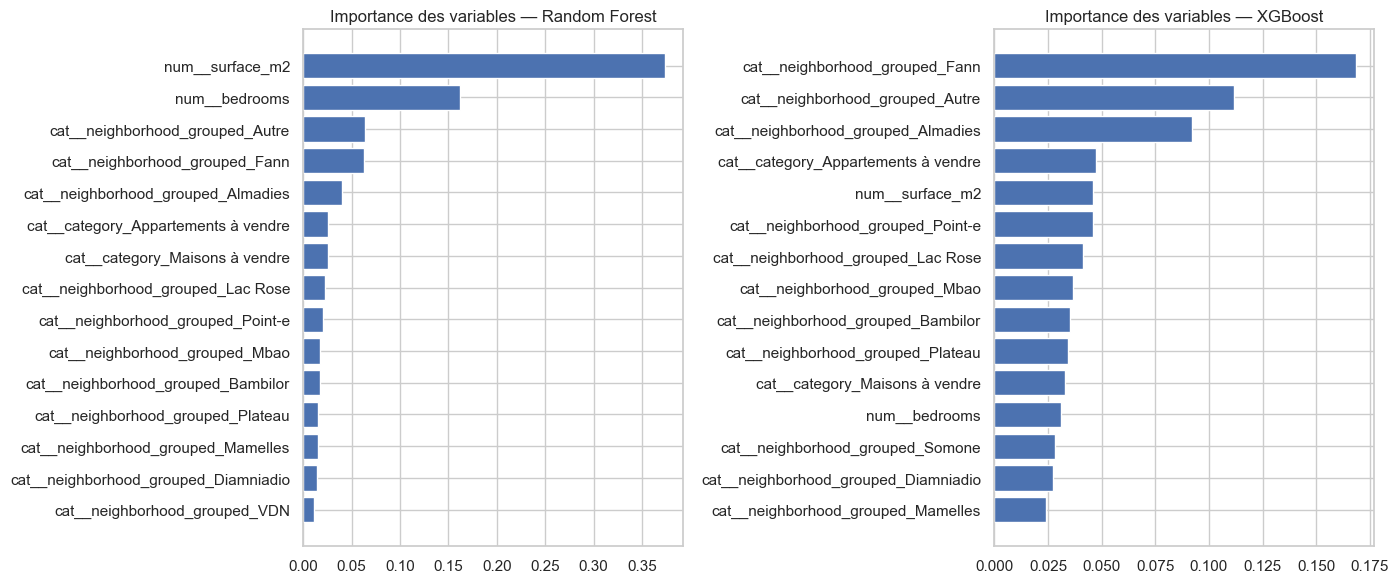
\includegraphics[width=0.95\textwidth]{figures/model_02.png}
  \caption{Importance des variables : Random Forest et XGBoost}
  \label{fig:feature-importance}
\end{figure}

L'analyse de l'importance des variables (Figure~\ref{fig:feature-importance}) confirme les
observations de l'analyse exploratoire : la surface est systématiquement la variable la plus
déterminante, suivie par les indicatrices de quartier les plus fréquentes (Almadies, Ngor,
Mermoz), tandis que le nombre de chambres contribue de façon plus marginale, cohérent avec sa
corrélation plus faible observée en Figure~\ref{fig:eda-corr}.

\subsubsection{Comparaison avec la littérature}

Les performances obtenues ($R^2 = 0{,}751$ pour le meilleur modèle) sont sensiblement
inférieures à celles rapportées par \citet{sharma2024optimal} sur le jeu de données Ames Housing
($R^2 \approx 0{,}89$). Cet écart s'explique principalement par deux facteurs : le volume de
données (603 contre plusieurs milliers d'observations pour Ames Housing) et surtout la richesse
des variables descriptives (4 variables mobilisées ici, contre 79 pour Ames Housing, incluant
l'âge du bien, la qualité des matériaux, l'état de la toiture, etc., absentes des annonces
Expat-Dakar). Le classement relatif des modèles (méthodes ensemblistes surpassant nettement la
régression linéaire) est en revanche cohérent avec \citet{truong2020housing} et
\citet{nwankwo2023lagos}.

Le fait que le MLP n'égale pas Random Forest est également cohérent avec les observations de
\citet{yazdani2021mldl} : sur un volume de données de l'ordre de quelques centaines
d'observations, les réseaux de neurones ne disposent généralement pas d'assez d'exemples pour
exprimer leur capacité de modélisation, contrairement aux méthodes ensemblistes à base
d'arbres, plus robustes dans ce régime de données.

\subsubsection{Discussion}

Plusieurs limites doivent être soulignées. \textbf{Premièrement}, la richesse des
caractéristiques disponibles est restreinte aux champs affichés systématiquement par
Expat-Dakar (surface, chambres, quartier, type). Des variables reconnues comme déterminantes
dans la littérature (âge du bien, état/qualité de construction, proximité des axes routiers ou
équipements, statut foncier (titre foncier ou non), un facteur pourtant mentionné dans plusieurs
titres d'annonces observées lors de la collecte) n'ont pas pu être exploitées de façon
structurée. \textbf{Deuxièmement}, la concentration géographique du jeu de données (85~\% des
annonces à Dakar) limite la capacité du modèle à généraliser sur le reste du territoire.
\textbf{Troisièmement}, les prix collectés sont des prix affichés, négociables par nature, et
non des prix de transaction effectivement conclus, ce qui introduit un bruit structurel
difficilement réductible sans accès à des données notariales.

\section{II. Outils de développement et de déploiement}

\subsection{Environnement de développement}

Le développement a été réalisé en Python, avec une phase d'exploration et de modélisation
menée sous forme de notebooks Jupyter, conçus pour être exécutés indifféremment en local ou sur
Google Colab (chargement des données avec repli automatique sur un import manuel si le fichier
n'est pas présent dans la session). L'éditeur Visual Studio Code a été utilisé pour le
développement du script de collecte et de l'application finale.

\subsection{Technologies de développement}

\begin{itemize}
  \item \textbf{Collecte de données :} \texttt{requests} et \texttt{BeautifulSoup} (analyse et
  extraction HTML).
  \item \textbf{Traitement de données :} \texttt{pandas}, \texttt{numpy}.
  \item \textbf{Modélisation :} \texttt{scikit-learn} \citep{pedregosa2011scikitlearn}
  (régression linéaire, Random Forest, MLP, pipelines de prétraitement, recherche
  d'hyperparamètres), \texttt{xgboost} \citep{chen2016xgboost}.
  \item \textbf{Visualisation :} \texttt{matplotlib}, \texttt{seaborn} (notebooks),
  \texttt{plotly} (interface interactive).
  \item \textbf{Interface graphique :} \texttt{Streamlit}.
  \item \textbf{Persistance des modèles :} \texttt{joblib}.
\end{itemize}

\subsection{Architecture de la solution}

Le pipeline du projet est organisé en quatre étapes séquentielles et indépendantes,
matérialisées par autant de composants :

\begin{enumerate}
  \item \texttt{src/scraper.py} : collecte les annonces et produit\\
  \url{data/raw/expat_dakar_listings_raw.csv}.
  \item \texttt{notebooks/01\_eda\_nettoyage.ipynb} : nettoie les données et produit\\
  \url{data/processed/expat_dakar_listings_clean.csv}, accompagné des visualisations
  exploratoires.
  \item \texttt{notebooks/02\_modelisation.ipynb} : encode les variables, entraîne et optimise
  les quatre modèles, puis sauvegarde les pipelines entraînés (\texttt{models/*.joblib}) ainsi
  qu'un fichier de métadonnées (\texttt{models/metadata.json}) décrivant les catégories
  disponibles, les plages de valeurs et les performances de chaque modèle.
  \item \texttt{app.py} : application Streamlit consommant les modèles et métadonnées
  sauvegardés pour proposer prédiction, exploration des données et comparaison des modèles.
\end{enumerate}

Chaque modèle est encapsulé dans un \emph{pipeline} scikit-learn intégrant le prétraitement
(mise à l'échelle des variables numériques, encodage \emph{one-hot} des variables
catégorielles) et l'estimateur, garantissant que les mêmes transformations sont appliquées de
façon identique à l'entraînement et à l'inférence dans l'application finale.

\subsection{Architecture et services du déploiement}

L'application est exécutable localement (\texttt{streamlit run app.py}) et a été déployée sur
\emph{Streamlit Community Cloud}. Un fichier \texttt{requirements.txt} liste les dépendances
nécessaires à la reproduction de l'environnement d'exécution.

\begin{itemize}
  \item \textbf{Lien d'accès :} \url{https://estimation-valeurs-immobilieres.streamlit.app/}
  \item \textbf{Code source :} \url{https://github.com/Laminito/MemoireM1DIT.git}
\end{itemize}

\section{Conclusion}

L'implémentation réalisée démontre la faisabilité d'un système d'estimation immobilière pour le
marché sénégalais à partir de données librement accessibles en ligne. Le modèle Random Forest
optimisé constitue la meilleure solution identifiée, avec des performances certes inférieures à
celles obtenues sur des jeux de données occidentaux plus riches, mais cohérentes avec l'état de
l'art compte tenu des contraintes de données propres au contexte sénégalais. L'architecture
modulaire retenue (collecte, nettoyage, modélisation, restitution) sépare clairement les
responsabilités et facilite l'évolution future de chaque composant, discutée en conclusion
générale.
